127. \begin{figure}[ht!]
\center{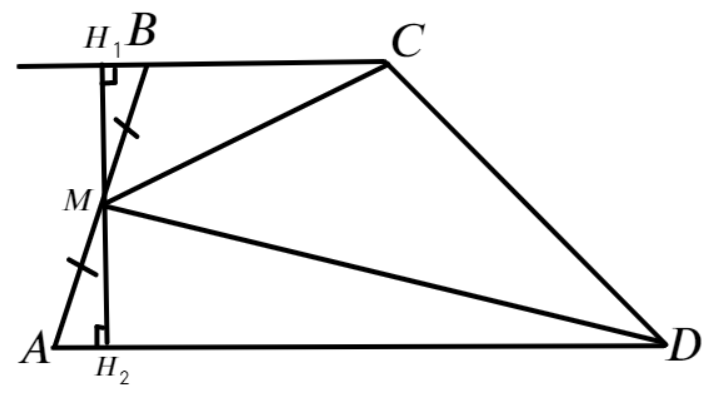
\includegraphics[scale=0.35]{g9-126.png}}
\end{figure}\\
Проведём через точку $M$ перпендикуляр к основаниям $H_1H_2.$ Треугольники $H_1MB$ и $H_2MA$ равны по гипотенузе и острому углу ($AM=MB,$ углы $AMH_2$ и $BMH_1$ вертикальные), значит $MH_1=MH_2.$ Тогда $S_{\Delta MBC}+S_{\Delta MAD}=\cfrac{1}{2}\cdot MH_1\cdot BC+\cfrac{1}{2}\cdot MH_2\cdot AD=\cfrac{1}{2}MH_1(BC+AD)=
\cfrac{1}{2}\cdot\cfrac{1}{2}H_1H_2(BC+AD)=\cfrac{1}{2}S_{ABCD}.$ Значит, $S_{\Delta MCD}=S_{ABCD}-(S_{\Delta MBC}+S_{\Delta MAD})=\cfrac{1}{2}S_{ABCD}=\cfrac{1}{2}\cdot26=13\text{ см}^2.$\\
